\section{SNF-Bench Design}
\label{sec:benchmark}

SNF-Bench evaluates long-horizon generation under a deliberately constrained setting: a fixed camera observing a scene containing both stationary structure and persistent natural motion. This isolates two failure modes that are difficult to separate in unconstrained video---\emph{static drift}, where nominally stationary structure moves over time, and \emph{flow decay}, where intended dynamics weaken or disappear. Every sequence is treated as a composition of two spatial roles, $\Omega_{\mathrm{static}}$ for regions expected to remain geometrically stationary and $\Omega_{\mathrm{flow}}$ for regions expected to exhibit sustained motion. The partition defines an evaluation role, not a semantic ontology: a riverbank is static support while the river surface is flow; buildings are static support in a rainfall scene while the falling rain is flow. SNF-Bench does not require dynamics inside $\Omega_{\mathrm{flow}}$ to follow any physical model. It measures whether motion stays localised to the appropriate regions and persists over time without contaminating static support.

Every system receives identical conditioning per item, and no prompt is rewritten for a particular method. Both conditioning modalities are evaluated under the same decomposition, differing only in how static support is established: the text-conditioned setting builds it in the opening of the sequence, while the image-conditioned setting takes it from a shared source image, so divergence there is attributable to the system rather than to a differently imagined scene. The main text reports the text-conditioned track for space; complete image-conditioned results appear in the supplementary material.

\subsection{Scene Categories and Horizons}
\label{sec:categories}

Prompts are stratified across representative fixed-camera natural processes---channel water, ocean waves, precipitation, fire and smoke, lava, and wind-borne motion---with the category set fixed before the final sweep. The strata are not equally populated: channel water accounts for \SNFtopCatShare\% of the principal prompt set, which is why every reported aggregate is macro-averaged over the \SNFnCategories{} categories rather than averaged over prompts, so that no single medium determines a headline value. Complete per-category counts are given in the supplementary material.

Four temporal regimes are used: $5$\,s as an initialisation check, $60$\,s as the reported horizon, and $120$ and $240$\,s as diagnostic tiers. Conclusions rest on the $60$\,s tier, which carries \SNFnPromptsSixty{} prompts; the longer tiers are reported in the supplementary material, since their samples do not support method-level separation on their own. A system that cannot reach a horizon under its released configuration is reported as unsupported rather than silently modified.

\subsection{Region Partition}
\label{sec:masks}

The partition is obtained automatically and identically for every sequence. Mean optical-flow magnitude over the leading $12\%$ of sampled frame pairs is thresholded by Otsu's method~\cite{otsu1979threshold} into a dynamic region and its complement; the static region is then eroded and a $4\%$ frame border discarded, which together form an ignored transition band so that boundary pixels---where the partition is least certain and flow least reliable---contribute to neither region.

Restricting the estimate to an early window is what prevents the measurement from becoming circular. Deriving a partition from a sequence's entire motion field would allow accumulated background drift to be read as evidence that the affected region is dynamic; at the $60$\,s horizon the partition is instead fixed from the first $7.1$\,s, before long-horizon drift has accumulated, and the metrics are evaluated over the remainder. The partition therefore reflects each system's spatial layout, which is unavoidable when every system authors its own scene, but it is not defined by the temporal failure being measured.

Two limitations follow, and both bound the conclusions drawn later. The partition is automatic rather than annotated, so a system that drifts within the first $12\%$ of its rollout can influence its own partition; we therefore treat partitions as measured quantities and recompute every result under systematic erosion and dilation of the boundary (Sec.~\ref{sec:validation}). And a two-way partition cannot represent layered content: rain and snow transit static support, so those pixels are assigned to one region by flow magnitude alone and static-fidelity values in precipitation scenes carry an additional unmodelled contribution. Derivation details, the sensitivity study, and the annotation protocol we regard as the natural strengthening of this component are given in the supplementary material.

\subsection{Benchmark Manifest}
\label{sec:manifest}

SNF-Bench is defined by a versioned manifest fixed before the final sweep, recording per item: identifier and category, exact prompt, target horizons, resolution and frame-rate metadata, and provenance. After freezing, items are never removed because a system performs poorly; corrections require a new benchmark version. A failure taxonomy---unsupported horizon, out-of-memory, runtime crash, numerical corruption, invalid output---is likewise fixed in advance, and failures are reported alongside successful generations rather than silently excluded. Coverage is counted from valid per-video measurements rather than from the presence of a results file, so a run that terminated early is reported as partial.

\begin{figure}[t]
\centering
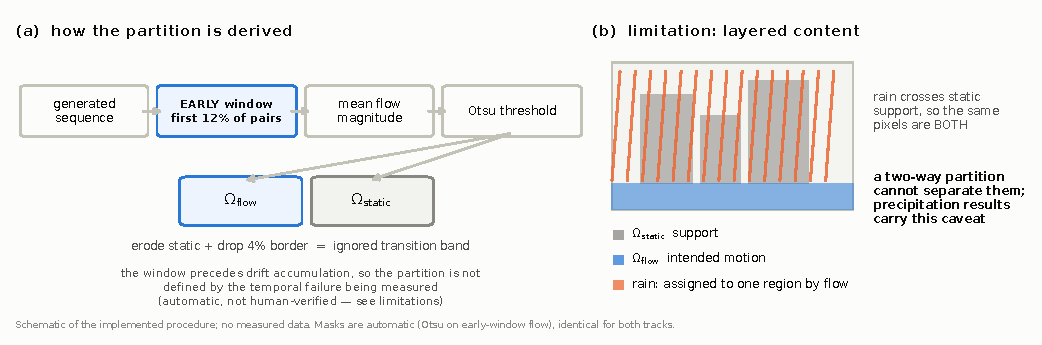
\includegraphics[width=\linewidth]{figures/fig2_mask_protocol.pdf}
\caption{\textbf{Region-partition protocol.} (a)~The partition is derived automatically from early-window flow, with an ignored transition band at the boundary. (b)~A two-way partition cannot represent layered content such as rain crossing static support.}
\label{fig:mask_protocol}
\end{figure}
